% =====================================================================
%  第 2.7 节 与第 3 节  旁注 · 用二次量子化证明 A∞ 关系式（原书 p.14–20）
% =====================================================================
\subsection{旁注：$\Mor(F_a,F_a)$ 的其它可能模型}\label{sec:2.7}

\begin{takeaway}
\begin{itemize}
  \item \textbf{物理图像}：对象到自身的态射空间可以另取模型，或用微分形式，或用奇异上链。前者让复合处处有定义，后者让余边界算子与 cup 积处处有定义。
  \item \textbf{数学工具}：de Rham dg 代数 $\Omega^\bullet(X)$、积分公式~\eqref{eq:29}、奇异上链复形 $C^\bullet_{\mathrm{sing}}(X,\mathbb Z)$、cup 积。
  \item \textbf{主要结论}：两个变体各有代价，前者丢掉整结构与计数味道，后者仍只给出部分定义的复合；只有链模型保留计数几何。
\end{itemize}
\end{takeaway}

(i) 可以考虑 $\Ainf$ 范畴 $\mathbb{F}$ 的一个变体 $\mathbb{F}_\Omega$：其中对象的自同态空间 $\Mor(F_a,F_a)$ 取为 de Rham dg 代数 $\Omega^\bullet(X)$。复合映射按式~\eqref{eq:4} 定义，只把链 $Z_{\alpha,a}$ 换成微分形式 $\omega_{\alpha,a}\in\Omega^\bullet(X)$，把系数 $\#\mathcal M$ 按积分公式~\eqref{eq:29} 定义（代替第~\ref{sec:2.1} 节的计数定义），并把 $\delta_{Z_q}$ 换成光滑形式 $\omega_q$。好处在于：只要函数 $F_a$ 处于一般位置，所得的 $\Ainf$ 范畴 $\mathbb{F}_\Omega$ 中复合就总有定义。代价是整结构丢失：态射空间与复合都是 $\mathbb R$ 上的上链复形，而不是 $\mathbb Z$ 上的。此外，复合的计数味道在这个模型里也丢掉了。我们还要指出：把 $\mathbb{F}_\Omega$ 中的复合限制到链的 $\epsilon$-光滑化 delta 形式上，就得到 $\mathbb{F}$ 中的复合。

% [Tutor Note: 这里三类 $\delta$ 的含义不同：$\delta_{Z_q}$ 是链的 delta 形式（对链积分即数交点），$\delta_{\mathrm{Unstab}_{P_{a_ia_{i+1}}}}$ 与 $\delta_{\mathrm{Stab}_{P_{a_1a_r}}}$ 是稳定、不稳定流形的 delta 形式，而 $\epsilon$-光滑化 delta 形式是链的 delta 形式的正则化。把三类混为一谈，就会误以为链与临界点在这个变体里地位相同。]

(ii) 另一种方案是把对象的自同态空间定义为奇异上链而非链，即 $\Mor(F_a,F_a)=C^\bullet_{\mathrm{sing}}(X,\mathbb Z)$，其 dg 代数结构由余边界算子与 cup 积给出。\footnote{P.~M. 感谢 Stephan Stolz 提出这一点。}这些运算总有定义，不需要额外的横截性要求。然而，要定义更一般的复合映射，仍需加上横截性要求。因此得到的仍是一个复合部分定义的 $\Ainf$ 范畴。

% [Tutor Note: 为什么 cup 积不需要横截性、而链的相交需要？cup 积是上链层面的代数运算，任意两条上链都可以相乘；链的相交则要求子流形横截，否则交点集不是离散的，计数无意义。但高阶复合仍要数 Morse 树与链的交，所以横截性没有消失，只是从基本运算挪到了复合这一步——这正是作者说「仍得到部分定义的范畴」的原因。]

\section{用二次量子化证明 $\Ainf$ 关系式}\label{sec:3}

\begin{takeaway}
\begin{itemize}
  \item \textbf{物理图像}：把范畴 $\mathbb{F}$ 的高阶复合看成某个 dg 代数经同伦转移得到的高阶乘法；在物理上，同一个结构就是 BF 理论的有效作用量，即二次量子化。
  \item \textbf{数学工具}：Morse 收缩与收缩三元组、Kontsevich--Soibelman 树形求和公式、Batalin--Vilkovisky 形式、奇辛纤维化上的纤维 BV 积分、Feynman 图展开。
  \item \textbf{主要结论}：诱导的乘法 $\mu$ 满足 $\Ainf$ 关系式~\eqref{eq:36}，由式~\eqref{eq:35} 即得范畴 $\mathbb{F}$ 的 $\Ainf$ 关系式~\eqref{eq:7}。BF 理论一侧的 $L_\infty$ 括号经式~\eqref{eq:47} 恢复 $\mu_n$，给出同一定理的场论证明。
\end{itemize}
\end{takeaway}

% [Tutor Note: 本节与第 4 节是定理~\ref{thm:1} 的两个独立证明。核心工具是同伦转移的存在性：给定收缩数据 $(i,\mathrm{p},K)$ 后，只要树形求和按次数逐次有限（Morse 收缩经正规化后满足这一条），dg 代数结构就能搬到 $\mathbb{M}$ 上。标准陈述是同调扰动引理，见 \cite{crainic,gugenheim,lambe}；树形求和的具体形状即 Kontsevich--Soibelman 公式 \cite{kontsevichsoibelman}。]

\subsection{同伦转移证明}\label{sec:3.1}

\begin{takeaway}
\begin{itemize}
  \item \textbf{物理图像}：把取值于微分形式的 $N\times N$ 矩阵 dg 代数收缩到 Morse 复形 $\mathbb{M}$，再用树的和定义高阶乘法，这就是同伦转移。
  \item \textbf{数学工具}：Morse 收缩式~\eqref{eq:20}、收缩三元组 $(\mathrm{i},\mathrm{p},K)$、Kontsevich--Soibelman 树形公式~\eqref{eq:33}。
  \item \textbf{主要结论}：诱导的 $\mu$ 与范畴复合 $m$ 逐项相等（式~\eqref{eq:35}，$\epsilon$ 对每个复合分别取充分小），于是 $\Ainf$ 关系式~\eqref{eq:36} 推出范畴关系式~\eqref{eq:7}。
\end{itemize}
\end{takeaway}

考虑如下微分分次（dg）代数：取 $X$ 上微分形式的超交换 de Rham dg 代数与 $N\times N$ 矩阵的结合代数 $M_N$ 的张量积。作为向量空间，它是
\[
V=\bigoplus_{a,b=1}^{N}\Omega_{ab},
\]
其中每个空间 $\Omega_{ab}$ 都同构于 $X$ 上微分形式的空间。现在，对 $a\neq b$，考虑（正规化）Morse 收缩：它把空间 $\Omega_{ab}$ 收缩到函数 $F_a-F_b$ 的 Morse 链上，其同伦取式~\eqref{eq:20}。于是得到 $V$ 到复形
\[
\mathbb{M}=\bigoplus_{a,b}\mathbb{M}_{ab},
\qquad\text{其中}\quad
\mathbb{M}_{ab}=
\begin{cases}
\mathrm{MC}(F_a-F_b,\mathbb{R}), & a\neq b,\\
\Omega_{aa}, & a=b
\end{cases}
\]
的收缩。

我们再次得到一个三元组，即嵌入、投影与链同伦：
\begin{equation}\tag{32}\label{eq:32}
K\;\curvearrowright\;V\ \underset{\mathrm{p}}{\overset{\mathrm{i}}{\rightleftarrows}}\ \mathbb{M},
\end{equation}
它们由 $(a,b)$-分块（$a\neq b$）上的正规化 Morse 收缩映射给出，在 $(a,a)$-分块上取平凡（$\mathrm{i}=\mathrm{p}=\mathrm{id}$，$K=0$）。

% [Tutor Note: 收缩三元组的标准条件是 $\mathrm{p}\,\mathrm{i}=\mathrm{id}_{\mathbb{M}}$ 与 $\mathrm{i}\,\mathrm{p}-\mathrm{id}_V=d_VK+Kd_V$（符号随分级约定略有出入），且 $K$ 的次数为 $-1$。$(a,a)$ 分块取 $\mathrm{i}=\mathrm{p}=\mathrm{id}$、$K=0$，是全篇「增强」的来源：$F_a-F_a\equiv0$ 没有 Morse 理论可用，故 $\Omega_{aa}$ 原样留在 $\mathbb{M}$ 中，不做 Morse 收缩。]

借助 Kontsevich--Soibelman 树形求和公式 \cite[第 6 章]{kontsevichsoibelman}，$V$ 上的 dg 代数结构同伦转移到 $\mathbb{M}$ 上，给出 $\mathbb{M}$ 上的一个 $\Ainf$ 代数结构。诱导的高阶乘法 $\mu\colon\mathbb{M}^{\otimes n}\to\mathbb{M}$ 如下给出：
\begin{equation}\tag{33}\label{eq:33}
\mu(X_1,\dots,X_n)=\sum_{T}\mu_T(X_1,\dots,X_n).
\end{equation}
其中：
\begin{itemize}
  \item $T$ 取遍（组合意义上的）$n$ 叶二叉有根树。
  \item $\mu_T\colon\mathbb{M}^{\otimes n}\to\mathbb{M}$ 是一个多线性映射，做法如下：用 $\mathrm{i}(X_i)$ 装饰树的第 $i$ 个叶，在每个内部顶点处计算 $V$ 中的乘积，在每条内部边上作用链同伦 $K$，最后在根处作用投影 $\mathrm{p}$。例如（下图为原书 p.15 的手绘树形图，按原式整行裁入，未重排）：
\begin{center}
  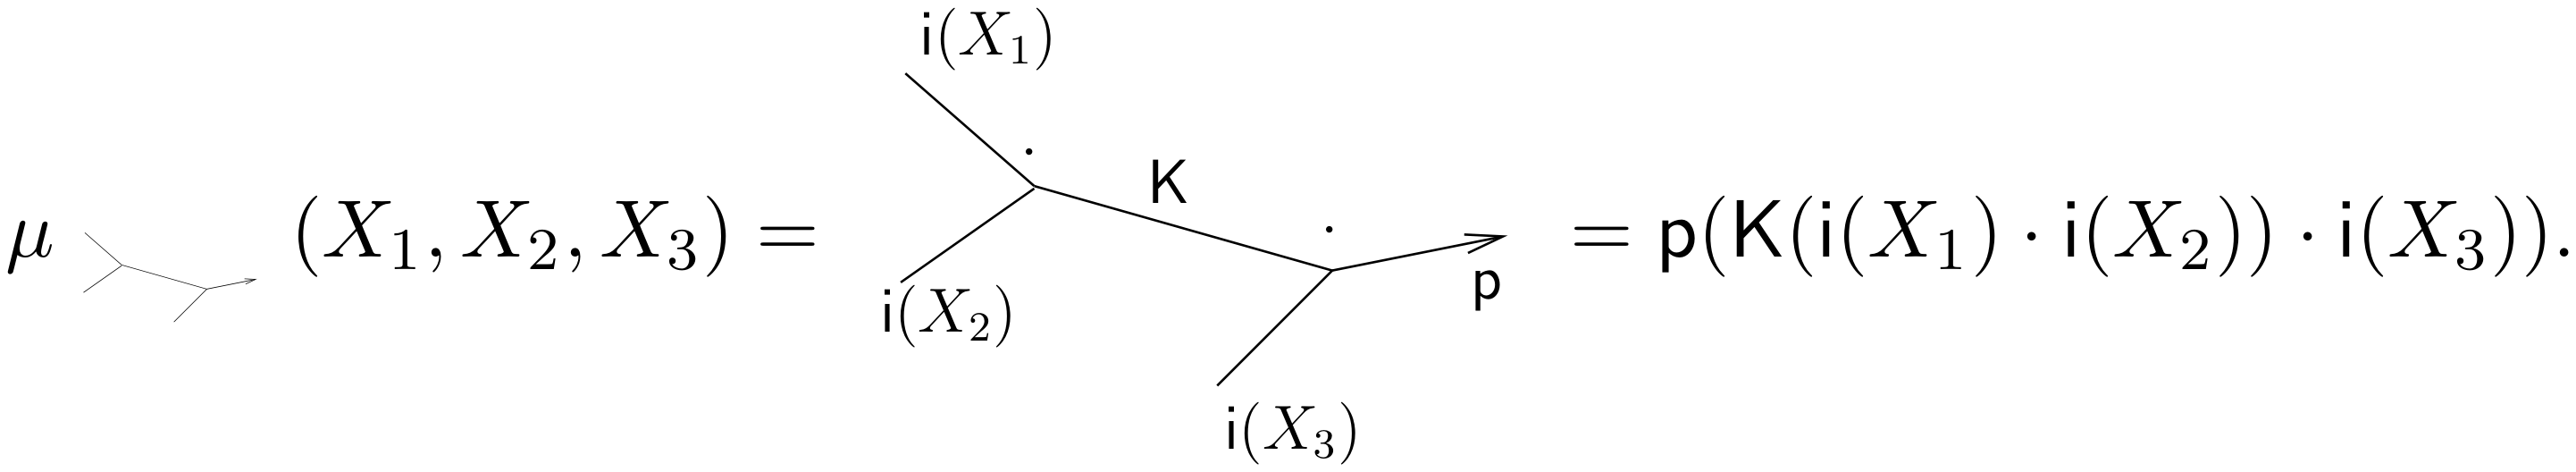
\includegraphics[width=0.86\linewidth]{figtree33.png}
\end{center}
% 上式在源码中的可编辑形式（供检索与改写；排版时由上面原图代替）：
% \mu(X_1,X_2,X_3)=\mathrm{p}\bigl(K(\mathrm{i}(X_1)\cdot \mathrm{i}(X_2))\cdot \mathrm{i}(X_3)\bigr).
\end{itemize}

% [Tutor Note: 次数核对：$n$ 叶二叉有根树有 $n-1$ 个内部顶点、$n-2$ 条内部边；乘积次数为 $0$，$K$ 的次数为 $-1$，故 $\mu_n$ 的次数为 $2-n$，与式~\eqref{eq:3} 中复合映射的次数一致。若把 $K$ 与乘积的次数记反，式~\eqref{eq:36} 的符号会整体错位。]
% [Tutor Note: 上式原书是手绘的二叉树（叶装饰 $\mathrm{i}(X_1),\mathrm{i}(X_2),\mathrm{i}(X_3)$，先由乘积合并前两个叶，在内部边上作用 $K$ 后再与第三个叶相乘，最后在根处作用 $\mathrm{p}$）。译文按原式整行裁图插入（图文件 \mbox{figtree33.png}），未重排；其组合型由「$n$ 叶二叉有根树」与上面的装饰规则唯一决定。]

这个诱导出的 $\mathbb{M}$ 上的 $\Ainf$ 代数结构与 $\Ainf$ 范畴 $\mathbb{F}$ 的关系如下。设给定一列可复合的态射
\begin{equation}\tag{34}\label{eq:34}
F_{a_1}\xrightarrow{x_1}F_{a_2}\xrightarrow{x_2}\cdots\xrightarrow{x_n}F_{a_{n+1}},
\end{equation}
其中当 $a_i\neq a_{i+1}$ 时，$x_i$ 是 $F_{a_i}-F_{a_{i+1}}$ 的临界点（更一般地，是 Morse 链）；当 $a_i=a_{i+1}$ 时，$x_i$ 是一条链。则
\begin{equation}\tag{35}\label{eq:35}
m(x_1,\dots,x_n)=\mu(X_1,\dots,X_n).
\end{equation}
左边是范畴 $\mathbb{F}$ 中的复合，右边是代数 $\mathbb{M}$ 中的高阶乘法。右边的输入取为：当 $a_i\neq a_{i+1}$ 时 $X_i=x_i$；当 $a_i=a_{i+1}$ 时 $X_i=\delta^{\epsilon}_{x_i}$，即链 $x_i$ 的 $\epsilon$-光滑化 delta 形式。我们把每个输入 $X_i$ 都理解为 $\mathbb{M}_{a_ia_{i+1}}$ 中的一个元素。等式~\eqref{eq:35} 对充分小的正规化参数 $\epsilon$ 成立，\footnote{不能为 $\mathbb{F}$ 中所有复合统一选取“充分小”的 $\epsilon$：$\epsilon$ 的界依赖于式~\eqref{eq:35} 中的输入链。归根结底，这是因为式~\eqref{eq:18} 中 $\epsilon$ 的界依赖于输入链。}并且由比较式~\eqref{eq:33} 与式~\eqref{eq:31}、式~\eqref{eq:4} 得到。\footnote{为完整起见我们指出，还有式~\eqref{eq:34} 中首、末对象重合的特殊情形，即 $a_1=a_{n+1}$。此时 $m(x_1,\dots,x_n)$ 是一条链（见第~\ref{sec:2.1} 节定理~\ref{thm:1} 之前的讨论），而 $\mu(X_1,\dots,X_n)$ 是该链的 $\epsilon$-光滑化 delta 形式。}

% [Tutor Note: $X_i$ 落在哪个分块极易记错：$a_i\neq a_{i+1}$ 时 $X_i=x_i$ 是 $\mathbb{M}_{a_ia_{i+1}}=\mathrm{MC}(F_{a_i}-F_{a_{i+1}})$ 中的临界点或 Morse 链；$a_i=a_{i+1}$ 时 $X_i=\delta^{\epsilon}_{x_i}$ 落在 $\Omega_{a_ia_i}$ 中。$\delta^{\epsilon}_{x_i}$ 不是临界点，必须当作光滑化 delta 形式才能进入树形公式~\eqref{eq:33}。]

\begin{thmenv}{注}{3.1}\label{rem:3.1}
在式~\eqref{eq:35} 中，Kontsevich--Soibelman 公式~\eqref{eq:33} 里一棵二叉有根树 $T$ 的贡献，对应式~\eqref{eq:31} 中一棵允许 2 价顶点的有根树 $T'$ 的贡献。这里 $T'$ 由 $T$ 去掉这样的 1 价顶点及其相邻边得到：该顶点的输入落在 $\mathbb{M}_{a_ia_{i+1}}$ 中，且 $a_i=a_{i+1}$。每一次这样的去除，都在 $T'$ 中生成一个 2 价顶点。
\end{thmenv}

% [Tutor Note: 这一步是式~\eqref{eq:33} 与式~\eqref{eq:31} 逐项对应的组合核心。式~\eqref{eq:31} 的树允许 2 价顶点来承载链 $Z_{\alpha,a}$；而式~\eqref{eq:33} 的二叉树叶在 $a_i=a_{i+1}$ 时带的是 $\delta^{\epsilon}_{x_i}$。截去这样的叶及其边，相当于把它并进 $\delta_{Z}$ 型因子，同时在 $T'$ 中留出一个 2 价顶点。图~\ref{fig:8} 给出的正是最简单的例子。]

\begin{figure}[htbp]
  \centering
  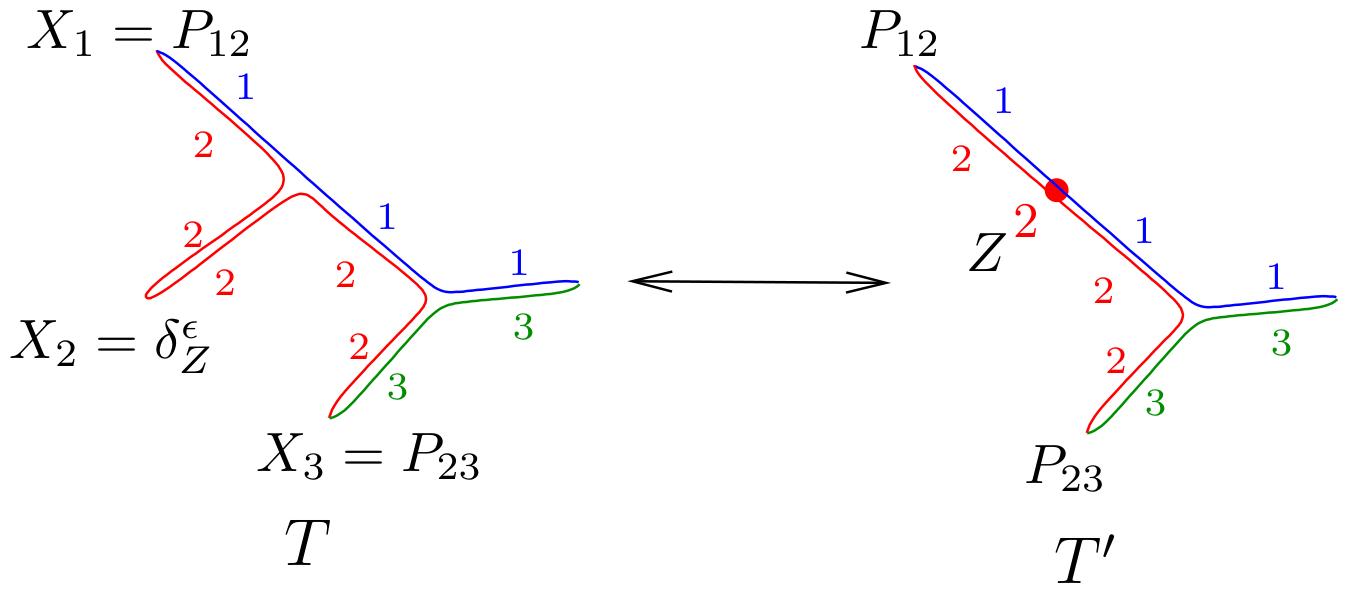
\includegraphics[width=\linewidth]{fig08.png}
  \caption{例：一个贡献到式~\eqref{eq:31} 的非二叉树，它由贡献到 Kontsevich--Soibelman 同伦转移公式的一个二叉树截去一个 $(aa)$-叶（图中 $a=2$）得到。图中明确标出了各边的双色。（原书 p.16）}
  \label{fig:8}
\end{figure}

由 Kontsevich--Soibleman 的一般结果 \cite{kontsevichsoibelman}，$\mathbb{M}$ 上诱导的高阶乘法 $\mu$ 满足 $\Ainf$ 代数关系式：
\begin{equation}\tag{36}\label{eq:36}
\sum_{r\ge0,\ s\ge1,\ r+s\le n}
\pm\,\mu\bigl(X_1,\dots,X_r,\ \mu(X_{r+1},\dots,X_{r+s}),\ X_{r+s+1},\dots,X_n\bigr)=0
\end{equation}
对任意输入 $X_1,\dots,X_n\in\mathbb{M}$ 成立。由式~\eqref{eq:35}，这蕴含 $\mathbb{F}$ 中复合映射的 $\Ainf$ 范畴关系式~\eqref{eq:7}。

% [Tutor Note: 原书 p.17 把 Soibelman 拼作 Soibleman，疑为笔误；译文照录，未擅改。读者应把它与 \cite{kontsevichsoibelman} 中的 Soibelman 认作同一人，切勿当成另一文献。]

\subsection{用 BF 理论有效作用量的进路}\label{sec:3.2}

\begin{takeaway}
\begin{itemize}
  \item \textbf{物理图像}：把上面的证明理解为 BF 理论的二次量子化：先写出 BV 形式下的 BF 作用量，再对非对角（快）场作纤维 BV 积分，得到只含对角慢场的有效作用量。
  \item \textbf{数学工具}：Batalin--Vilkovisky 形式、上三角矩阵代数 $\mathcal A$ 的正向极限、Nekrasov 型非对角轴规范、奇辛纤维化、Feynman 图展开。
  \item \textbf{主要结论}：有效作用量是 Feynman 树之和~\eqref{eq:41}，式~\eqref{eq:42} 给出前几项；BV 主方程~\eqref{eq:45} 等价于 $L_\infty$ 关系式~\eqref{eq:46}，再由式~\eqref{eq:47} 恢复 $\Ainf$ 乘法 $\mu_n$。
\end{itemize}
\end{takeaway}

上面所用的物理证明，可以用“二次量子化”来解释。也就是说，我们考虑 Batalin--Vilkovisky 形式下的 BF 理论\footnote{BV 形式下以非齐次微分形式为场的非阿贝尔 BF 理论，参看 \cite{cattaneo}。}，它由作用量
\begin{equation}\tag{37}\label{eq:37}
S=\int_X\Bigl\langle B,\ dA+\frac12[A,A]\Bigr\rangle
\end{equation}
定义。其中场 $A$ 是取值于李代数 $\mathfrak g=\mathfrak{gl}_N(\mathcal A)$ 的微分形式。这里 $\mathfrak g$ 是元素取自 $\mathcal A$ 的 $N\times N$ 矩阵构成的李代数；$\mathcal A$ 是 $\widetilde N\times\widetilde N$ 的上三角矩阵代数，其中 $\widetilde N$ 很大（更确切地说，我们取正向极限 $\widetilde N\to\infty$）。$B$ 是取值于 $\mathfrak g^*$ 的微分形式。

% [Tutor Note: 式~\eqref{eq:37} 有三层结构：$A$ 的矩阵指标在 $N\times N$ 上（对应 $\mathbb{F}$ 的 $N$ 个对象），每个矩阵元再取值于 $\mathcal A$（大型上三角矩阵代数）。$\langle\,,\rangle$ 是 $\mathfrak g$ 与 $\mathfrak g^*$ 的配对；对微分形式还要配上 wedge 积与矩阵迹，原文按标准 BF 记号省略未写。$A$ 是奇变量，故 $dA+\frac12[A,A]$ 就是曲率。]

\begin{thmenv}{注}{3.2}\label{rem:3.2}
若只考虑以 $N\times N$ 矩阵为系数的 BF 理论，那么通过有效作用量得到的将是 $\mathbb{M}$ 上的 $L_\infty$ 代数结构，即所需 $\Ainf$ 结构的反对称化。于是，用这样的系数会丢掉高阶乘法的一部分数据。为弥补这一点，我们让场的 $(a,b)$-分量取值于 $\mathcal A$，由此引入非交换性。这相当于先把 $\Ainf$ 代数 $\mathbb{M}$ 与 $\mathcal A$ 作张量积，再做反对称化。所得的 $\mathbb{M}\otimes\mathcal A$ 上的 $L_\infty$ 括号，能记住 $\mathbb{M}$ 上 arity 至多 $\widetilde N-1$ 的 $\Ainf$ 乘法 $\mu$，见下文式~\eqref{eq:47}。
\end{thmenv}

% [Tutor Note: 为何必须把系数扩成 $\mathcal A$：只取 $N\times N$ 矩阵时，反对称化后只能读到 $L_\infty$ 括号，$\Ainf$ 的 $\mu_n$ 被混同。张量 $\mathcal A$ 之后，矩阵单位 $t_{ij}$ 像「标签」一样把输入与输出的次序记下来（见式~\eqref{eq:47}）。再取正向极限 $\widetilde N\to\infty$，是为了不设 arity 的上限。$\mathcal A$ 幂零这一点，在「非幂零 $\mathfrak g$」那条脚注处会用到。]

我们把 $A$ 分解为对角场 $A_Z$（相对于 $M_N$ 因子）与非对角场 $A_W$。名称来自标准模型中的 $Z$、$W$ 规范玻色子。然后我们采用一个精巧版本的规范固定，它推广了轴规范（最早由 N.~Nekrasov 在与 A.~Losev 的私人通信中提出）：\footnote{注意通常的轴（或时间）规范是 $A_0=0$，即 $\iota_{\frac{\partial}{\partial t}}A=0$。这里推广的一个特点是：我们对规范场的不同分量取不同的向量场。}
\begin{equation}\tag{38}\label{eq:38}
\iota_{v_{ab}}(A_W)_{ab}=0,
\end{equation}
其中 $v_{ab}$ 是 $F_a-F_b$ 的梯度向量场。我们指出，这个规范条件等价于 Morse 链同伦式~\eqref{eq:12} 把 $(A_W)_{ab}$ 湮灭。

% [Tutor Note: 式~\eqref{eq:38} 把「几何」塞进了规范固定：$\iota_{v_{ab}}$ 是沿梯度场 $v_{ab}$ 的缩并。作者断言这个条件等价于「$(A_W)_{ab}$ 被 Morse 链同伦式~\eqref{eq:12} 湮灭」。结合下文 $\mathcal L=\mathrm{im}K\oplus\mathrm{im}K$，这条等价关系正是「几何规范固定转化为内部边装饰 $K$」的翻译词典，也是全节物理思想的关键一步。]

经过这样的规范固定，我们直接把场 $A_W$ 积掉，就得到只含 $A_Z$ 场与临界点的有效理论，而临界点是 $A_W$ 场的残余。

\textbf{更多细节.}\quad 有效作用量由纤维 BV 积分定义：
\begin{equation}\tag{39}\label{eq:39}
e^{\frac{i}{\hbar}S_{\mathrm{eff}}(A',B')}=\int_{\mathcal L}e^{\frac{i}{\hbar}S(A,B)},
\end{equation}
积分沿奇辛纤维化
\begin{equation}\tag{40}\label{eq:40}
\Omega^\bullet(X,\mathfrak g)[1]\oplus\Omega^\bullet(X,\mathfrak g^*)[\dim X-2]
\ \longrightarrow\
\mathbb{M}\otimes\mathcal A[1]\oplus\mathbb{M}\otimes\mathcal A^*[\dim X-2]
\end{equation}
的纤维中的一个 Lagrangian $\mathcal L$ 进行。左边是 BF 理论的 BV 场空间（其元素为对 $(A,B)$），右边是我们选定的“慢场”空间，其元素记作 $(A',B')$。式~\eqref{eq:40} 中的投影是 $\mathrm{p}\oplus\mathrm{p}$，由式~\eqref{eq:32} 的映射拼成，并按 $\mathcal A$-线性延拓；它也有截面 $\mathrm{i}\oplus\mathrm{i}$。式~\eqref{eq:40} 纤维中的 Lagrangian $\mathcal L$ 由规范固定条件~\eqref{eq:38} 确定，换言之由 $\mathcal L=\mathrm{im}K\oplus\mathrm{im}K$ 给出。

% [Tutor Note: 式~\eqref{eq:40} 两端的方括号是次数平移：$[1]$ 与 $[\dim X-2]$ 必须逐项对齐，混淆两者会破坏奇辛配对的次数。右端 $\mathbb{M}\otimes\mathcal A^*$ 中的星号是对 $\mathcal A$ 取对偶，不是对整个张量积取对偶。$\mathcal L=\mathrm{im}K\oplus\mathrm{im}K$ 说明纤维积分沿 $K$ 的像进行，故内部边最终由 $K$ 装饰。]

把纤维 BV 积分~\eqref{eq:39} 当作受扰高斯积分算出来，有效作用量就写成 Feynman 图之和：
\begin{equation}\tag{41}\label{eq:41}
S_{\mathrm{eff}}=\sum_{\Gamma}\frac{1}{|\mathrm{Aut}(\Gamma)|}\Phi_\Gamma(A',B').
\end{equation}
这里
\begin{itemize}
  \item 求和取遍二叉有根树 $\Gamma$（Feynman 图），按图同构类计。
  \item $|\mathrm{Aut}(\Gamma)|$ 是树 $\Gamma$ 的自同构群的阶。
  \item $\Phi_\Gamma(A',B')$ 是慢场空间（式~\eqref{eq:40} 的右端）上的多项式函数。它的做法是：用 $\mathrm{i}(A')$ 装饰 $\Gamma$ 的叶，用 $\langle B',\mathrm{p}(\cdots)\rangle$ 装饰根，用 dg 李代数 $\Omega^\bullet(X,\mathfrak g)$ 中的李括号装饰二叉顶点，用链同伦 $K$ 装饰内部边。
\end{itemize}

式~\eqref{eq:41} 的前几项是：
\begin{equation}\tag{42}\label{eq:42}
\begin{split}
S_{\mathrm{eff}}={}&
\langle B',d_{\mathbb{M}}A'\rangle
+\frac12\langle B',\mathrm{p}[\mathrm{i}(A'),\mathrm{i}(A')]\rangle
+\frac12\langle B',\mathrm{p}[K[\mathrm{i}(A'),\mathrm{i}(A')],\mathrm{i}(A')]\rangle\\
&+\frac12\langle B',\mathrm{p}[K[K[\mathrm{i}(A'),\mathrm{i}(A')],\mathrm{i}(A')],\mathrm{i}(A')]\rangle
+\frac18\langle B',[K[\mathrm{i}(A'),\mathrm{i}(A')],K[\mathrm{i}(A'),\mathrm{i}(A')]]\rangle+\cdots
\end{split}
\end{equation}

% [Tutor Note: 系数与 $|\mathrm{Aut}(\Gamma)|$ 对应：前三个单链树的权重是 $1/2$；最后的「哑铃」树两条 $K$ 边可交换，自同构群阶为 $8$，故系数是 $1/8$ 而不是 $1/4$。抄写式~\eqref{eq:42} 时最易在此出错，请对原书 p.18 第二行逐字核对。]

\textbf{用对角场与非对角场来描述.}\quad 可以把场（以及慢场）相对于 $M_N$ 因子分成对角分量与非对角分量：
\[
\begin{gathered}
A=A_Z+A_W,\qquad B=B_Z+B_W,\\
A'=A_Z+A'_W,\qquad B'=B_Z+B'_W.
\end{gathered}
\]
于是作用量~\eqref{eq:37} 成为
\begin{equation}\tag{43}\label{eq:43}
\begin{split}
S=\int_X&\,\underset{(a)}{\langle B_Z,dA_Z\rangle}
+\underset{(b)}{\langle B_W,dA_W\rangle}
+\underset{(c)}{\Bigl\langle B_W,\frac12[A_W,A_W]\Bigr\rangle}\\
&+\underset{(d)}{\langle B_W,[A_Z,A_W]\rangle}
+\underset{(e)}{\Bigl\langle B_Z,\frac12[A_Z,A_Z]\Bigr\rangle}
+\underset{(f)}{\Bigl\langle B_Z,\frac12[A_W,A_W]\Bigr\rangle}.
\end{split}
\end{equation}
场 $A_Z,B_Z$ 是非动力学的：在式~\eqref{eq:39} 中不对它们积分；而 $A_W,B_W$ 是动力学场。在式~\eqref{eq:43} 中：
\begin{itemize}
  \item 项 (a)、(e) 是常数。
  \item (b) 是动力学场的动能项，它产生分配给各条边的“传播子”$K$。
  \item (c) 产生一个三价“相互作用”顶点（两条入半边与一条出半边）。
  \item (d) 产生一个三价顶点，带一条自由的（或“外部的”）入半边，其装饰为 $A_Z$。
  \item (f) 产生一个三价顶点，带一条自由的出半边，其装饰为 $B_Z$。
  \item 带 $A_W$ 的半边既可以是外部的（装饰为 $A'_W$），也可以是内部的（对应于该场分量的快部分、即动力学部分）。内部半边与一条内部的 $B_W$ 半边相连，所得的内部边由传播子装饰。类似地，$B_W$ 半边可以是外部的，也可以是内部的。
\end{itemize}

% [Tutor Note: 六项分工要记清：(b)(c) 只含 $A_W$，给出传播子与三价相互作用；(a)(e) 不含 $A_W$，在纤维积分中是常数；(d)(f) 各带一条 $A_Z$ 或 $B_Z$ 的外线，把慢场接到动力学部分。注意 (e) 与 (f) 的被积式都含 $\frac12[\cdot,\cdot]$，但 (e) 是常数项、(f) 是外线顶角，切勿记反。]

\begin{figure}[htbp]
  \centering
  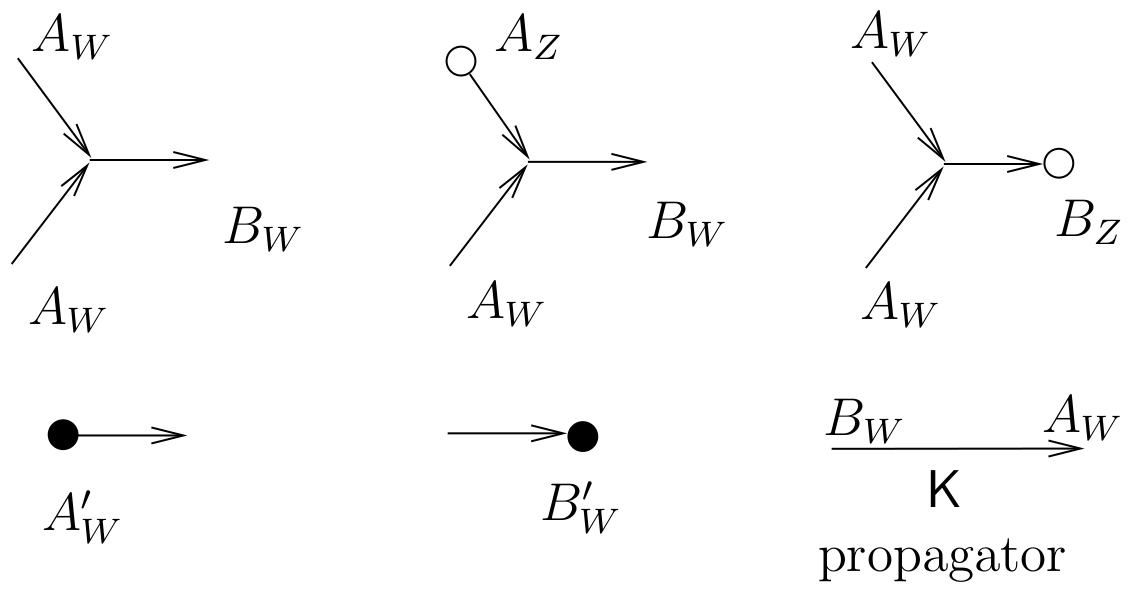
\includegraphics[width=0.9\linewidth]{fig09.png}
  \caption{Feynman 规则（Feynman 图的构件）。（原书 p.19）}
  \label{fig:9}
\end{figure}

\begin{figure}[htbp]
  \centering
  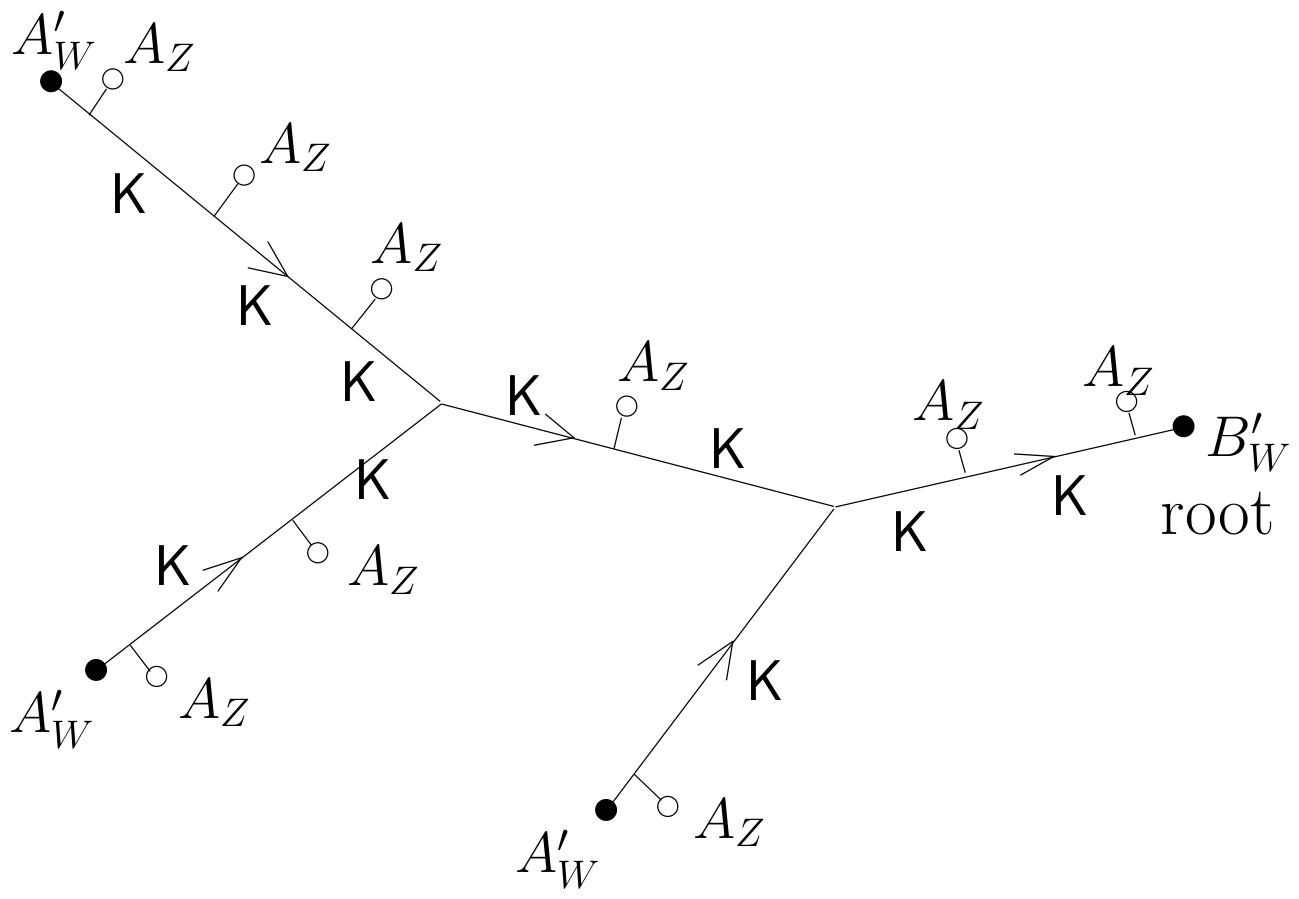
\includegraphics[width=0.9\linewidth]{fig10.png}
  \caption{一个贡献到 $S_{\mathrm{eff}}$ 的典型 Feynman 树，图中明确画出了场的对角部分与非对角部分。（原书 p.19）}
  \label{fig:10}
\end{figure}

把叶数相同的 Feynman 树的贡献归并起来，可以把 $S_{\mathrm{eff}}$ 写成
\begin{equation}\tag{44}\label{eq:44}
S_{\mathrm{eff}}=\sum_{n\ge1}\frac{1}{n!}\langle B',l_n(A',\dots,A')\rangle,
\end{equation}
其中 $l_n\colon\wedge^n(\mathbb{M}\otimes\mathcal A)\to\mathbb{M}\otimes\mathcal A$ 是由 $n$ 叶 Feynman 树给出的斜对称多线性运算。按 Feynman 图展开~\eqref{eq:41}，$l_n$ 可以写成非平面（或按同构类计的）二叉有根树之和，这是 Kontsevich--Soibelman 公式~\eqref{eq:33} 的李代数版本。我们指出，虽然一般地 BF 理论的有效作用量含有单圈图，但在我们这里它们消失，因为系数李代数 $\mathfrak g$ 幂零。\footnote{事实上，考虑非幂零的 $\mathfrak g$ 是很有意思的。例如取 $\mathcal A$ 为所有 $\widetilde N\times\widetilde N$ 矩阵的代数，这样有效作用量中会出现非平凡的单圈图。把它们理解为 Fukaya--Morse 范畴的“圈增强”，是作者们正在进行的工作。}

% [Tutor Note: $1/n!$ 来自 $n$ 个等价输入 $A'$ 的置换（$l_n$ 斜对称，$n!$ 个置换给出同一项）。按叶数归并式~\eqref{eq:41} 时，这个因子必须与树的同构群阶数一起核对，否则会差整数倍。]

我们要强调：按规范理论的逻辑，我们在为快场（慢场的补）上的积分~\eqref{eq:39} 选取规范固定。在 BV 形式中，这相当于在快场中选一个 Lagrangian 子空间；把积分改写成 Feynman 图之和时，这个子空间就对应传播子（即对边的装饰）。于是，我们的几何规范固定对应于“边被 Morse 链同伦式~\eqref{eq:12} 装饰”，而这又使得（在此规范下算出的）有效作用量与 Morse 树的计数相关。

% [Tutor Note: 这一段是全节的物理枢纽，值得慢读：规范固定（几何条件）→ 传播子（Feynman 规则里的边装饰）→ Morse 链同伦 $K$（组合数据）→ Morse 树计数（范畴的复合）。四个对象其实是同一件事的四种语言，作者用「规范理论的逻辑」把它们串成一条链。若省略这一步，读者会误以为 BF 有效作用量与 Morse 树计数只是碰巧形式相似。]

作用量~\eqref{eq:37} 满足 BV 主方程 $\{S,S\}=0$，这是 $\mathfrak g$-值形式的 dg 李代数中二次关系式 $d^2=0$、Leibniz 法则与 Jacobi 恒等式的推论。这里 $\{\,,\}$ 是与场空间上奇辛形式相伴的 Poisson 括号。因此，由纤维 BV 积分的 BV--Stokes 定理，有效作用量也满足主方程
\begin{equation}\tag{45}\label{eq:45}
\{S_{\mathrm{eff}},S_{\mathrm{eff}}\}=0.
\end{equation}
它等价于运算 $l_n$ 上的 $L_\infty$ 代数二次关系式：
\begin{equation}\tag{46}\label{eq:46}
\sum_{r\ge0,\ s\ge1,\ r+s=n}\frac{1}{r!\,s!}\sum_{\sigma\in S_n}
\pm\,l_{r+1}\bigl(y_{\sigma(1)},\dots,y_{\sigma(r)},l_s(y_{\sigma(r+1)},\dots,y_{\sigma(n)})\bigr)=0,
\end{equation}
其中 $y_1,\dots,y_n\in\mathbb{M}\otimes\mathcal A$ 是输入，$\sigma$ 取遍置换。关于通过纤维 BV 积分作 $L_\infty$ 代数的同伦转移，读者可参看 \cite{mnev}。

% [Tutor Note: 式~\eqref{eq:46} 与式~\eqref{eq:36} 的求和范围不同：这里 $r+s=n$，$n$ 个输入由置换 $\sigma$ 分配进内外两个括号，全部参与；而 $\Ainf$ 的式~\eqref{eq:36} 允许 $r+s\le n$，尾部可有剩余输入。照抄式~\eqref{eq:36} 的范围会漏项。]

\textbf{从 $L_\infty$ 回到 $\Ainf$.}\quad 我们可以从 $L_\infty$ 括号 $l_n$ 恢复 $\mathbb{M}$ 中的 $\Ainf$ 乘法（从而恢复 $\mathbb{F}$ 中的高阶复合）如下：
\begin{equation}\tag{47}\label{eq:47}
l_n(X_1\otimes t_{12},\dots,X_n\otimes t_{n,n+1})=\mu_n(X_1,\dots,X_n)\otimes t_{1,n+1},
\end{equation}
其中 $t_{ij}\in\mathcal A$ 是在 $(i,j)$ 位置为 $1$、其余元素为零的矩阵。这里 $X_i$ 是 $\mathbb{M}_{a_ib_i}$ 中的元素，我们要求 $b_i=a_{i+1}$（否则式~\eqref{eq:47} 两端都为零）。

% [Tutor Note: $t_{ij}$ 是上三角矩阵代数 $\mathcal A$ 中的矩阵单位。取 $t_{12},t_{23},\dots,t_{n,n+1}$ 是沿态射链 $(a_1,a_2),\dots,(a_n,a_{n+1})$ 把指标串起来，输出恰好落在 $t_{1,n+1}$ 上。若 $b_i\neq a_{i+1}$，乘积在 $\mathcal A$ 中为零，式~\eqref{eq:47} 两端同时消失。这正是 $\mathcal A$ 能「记住」$\Ainf$ 复合的组合机制。]
\endinput
